\section{Update with 2017 data-taking periods}
\label{sec:strong:r21}

The mild excess observed in the multi-bin region SR-0L-HH motivated checking the results with the 2017 data-taking periods 
as soon as they have become available. 
The analysis has been reproduced with all the data collected by the \gls{atlas} experiment in 2015, 2016 and 2017, 
for a total integrated luminosity of 79.8 \ifb. 
Both the cut-and-count and multi-bin regions have been updated in Ref. \cite{ATLAS-CONF-2018-041}, 
but in this section we present only the results 
of the multi-bin regions, since the main purpose is the follow up of the excess in the analysis of the 2015-2016 data.
Differences in the object definition that occurred due to a change in the \gls{atlas} software release between the 
two analyses are not discussed in this section and do not impact sensibly the physics results, more details can be found 
in Ref. \cite{ATLAS-CONF-2018-041}.


\subsection{Results}

The results of the fit in the \glspl{cr} extrapolated to the \glspl{vr} and \glspl{sr} are shown in Figures 
\ref{fig:pullVR_R21} and \ref{fig:pullSR_R21} respectively. 
We can see that there is good agreement with the predicted background in the \glspl{vr}, and the \glspl{vr} do now show any 
significant deviation from the expectations. 
In particular, the excess in SR-0L-HH is no longer present. 

\begin{figure}[htbp]
	\centering
	\subfigure[]{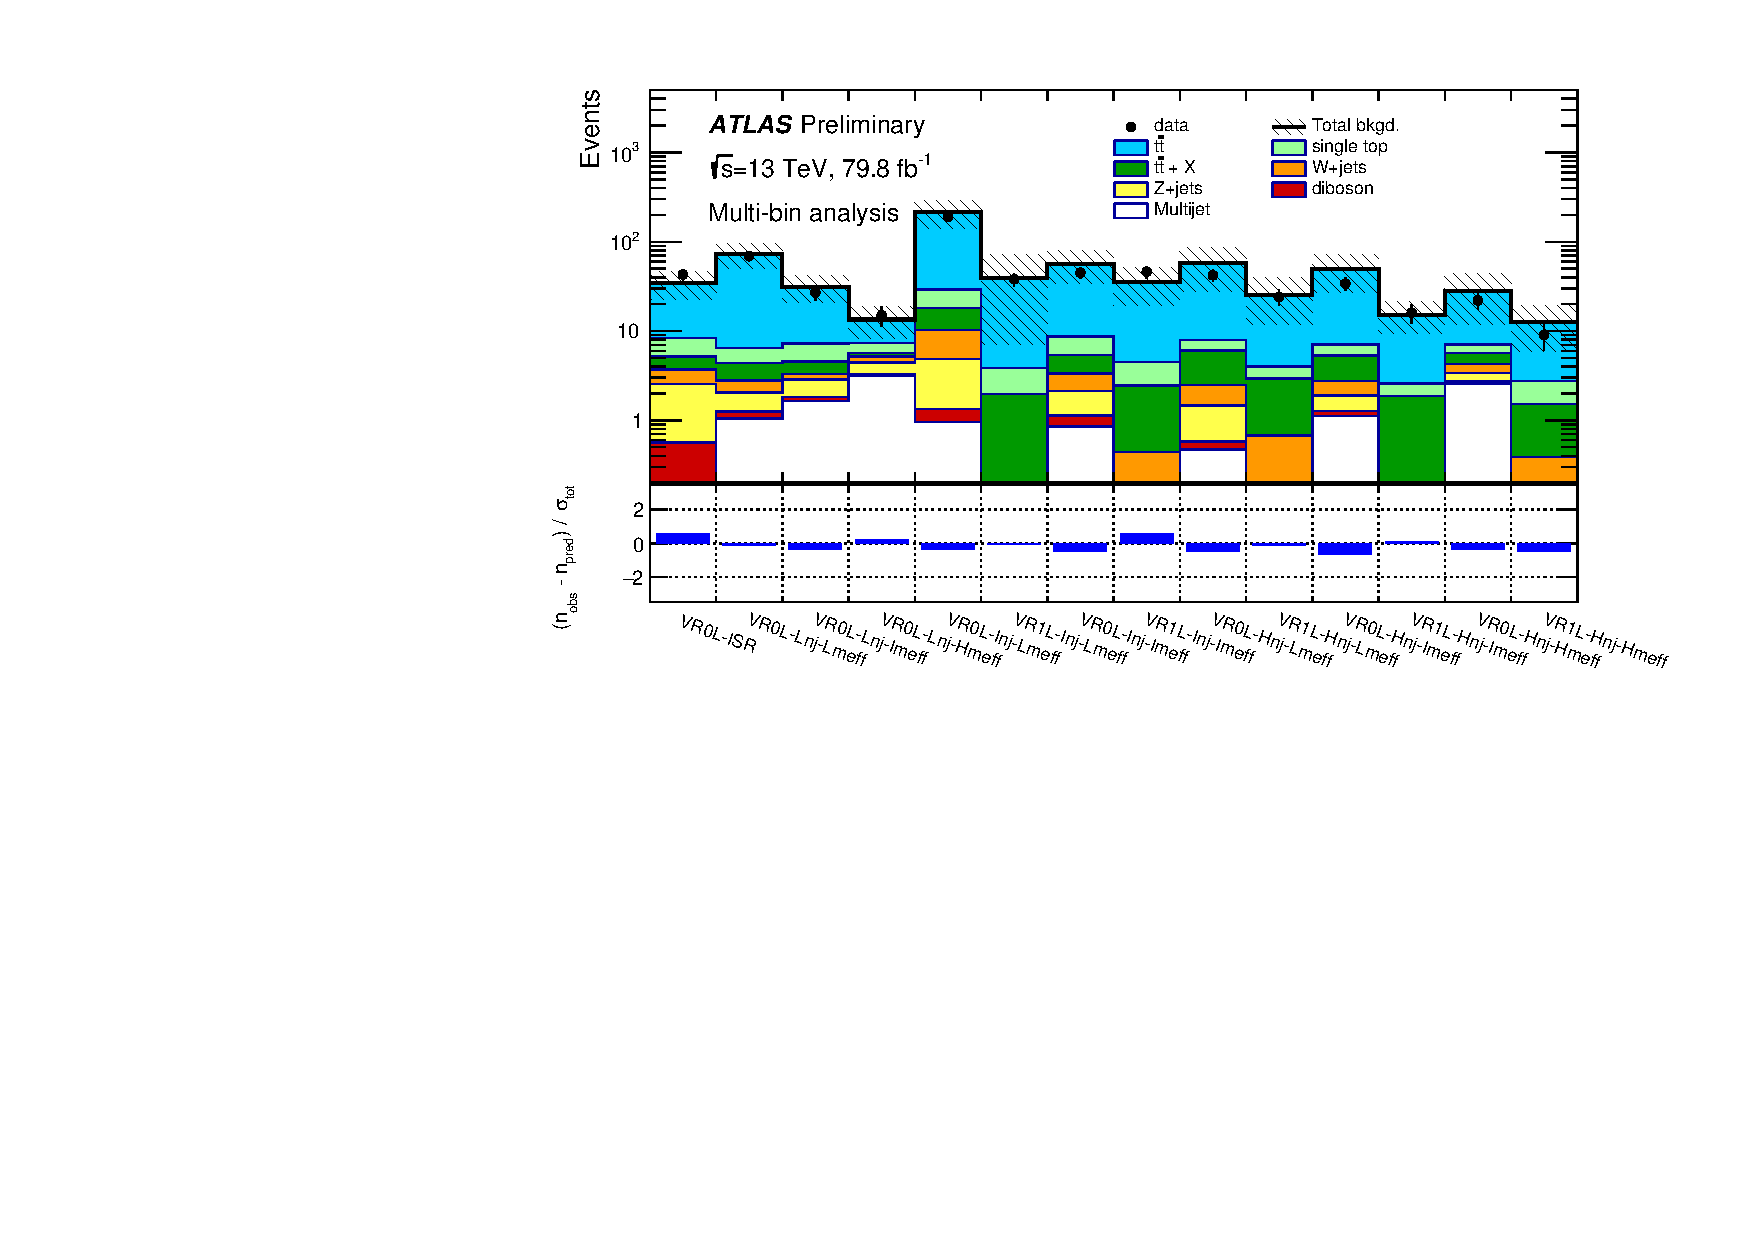
\includegraphics[width=0.9\textwidth]{figures/strong_prod/R21/multibin/histpull_grouping_VR.pdf}\label{fig:pullVR_R21}}\\
	\subfigure[]{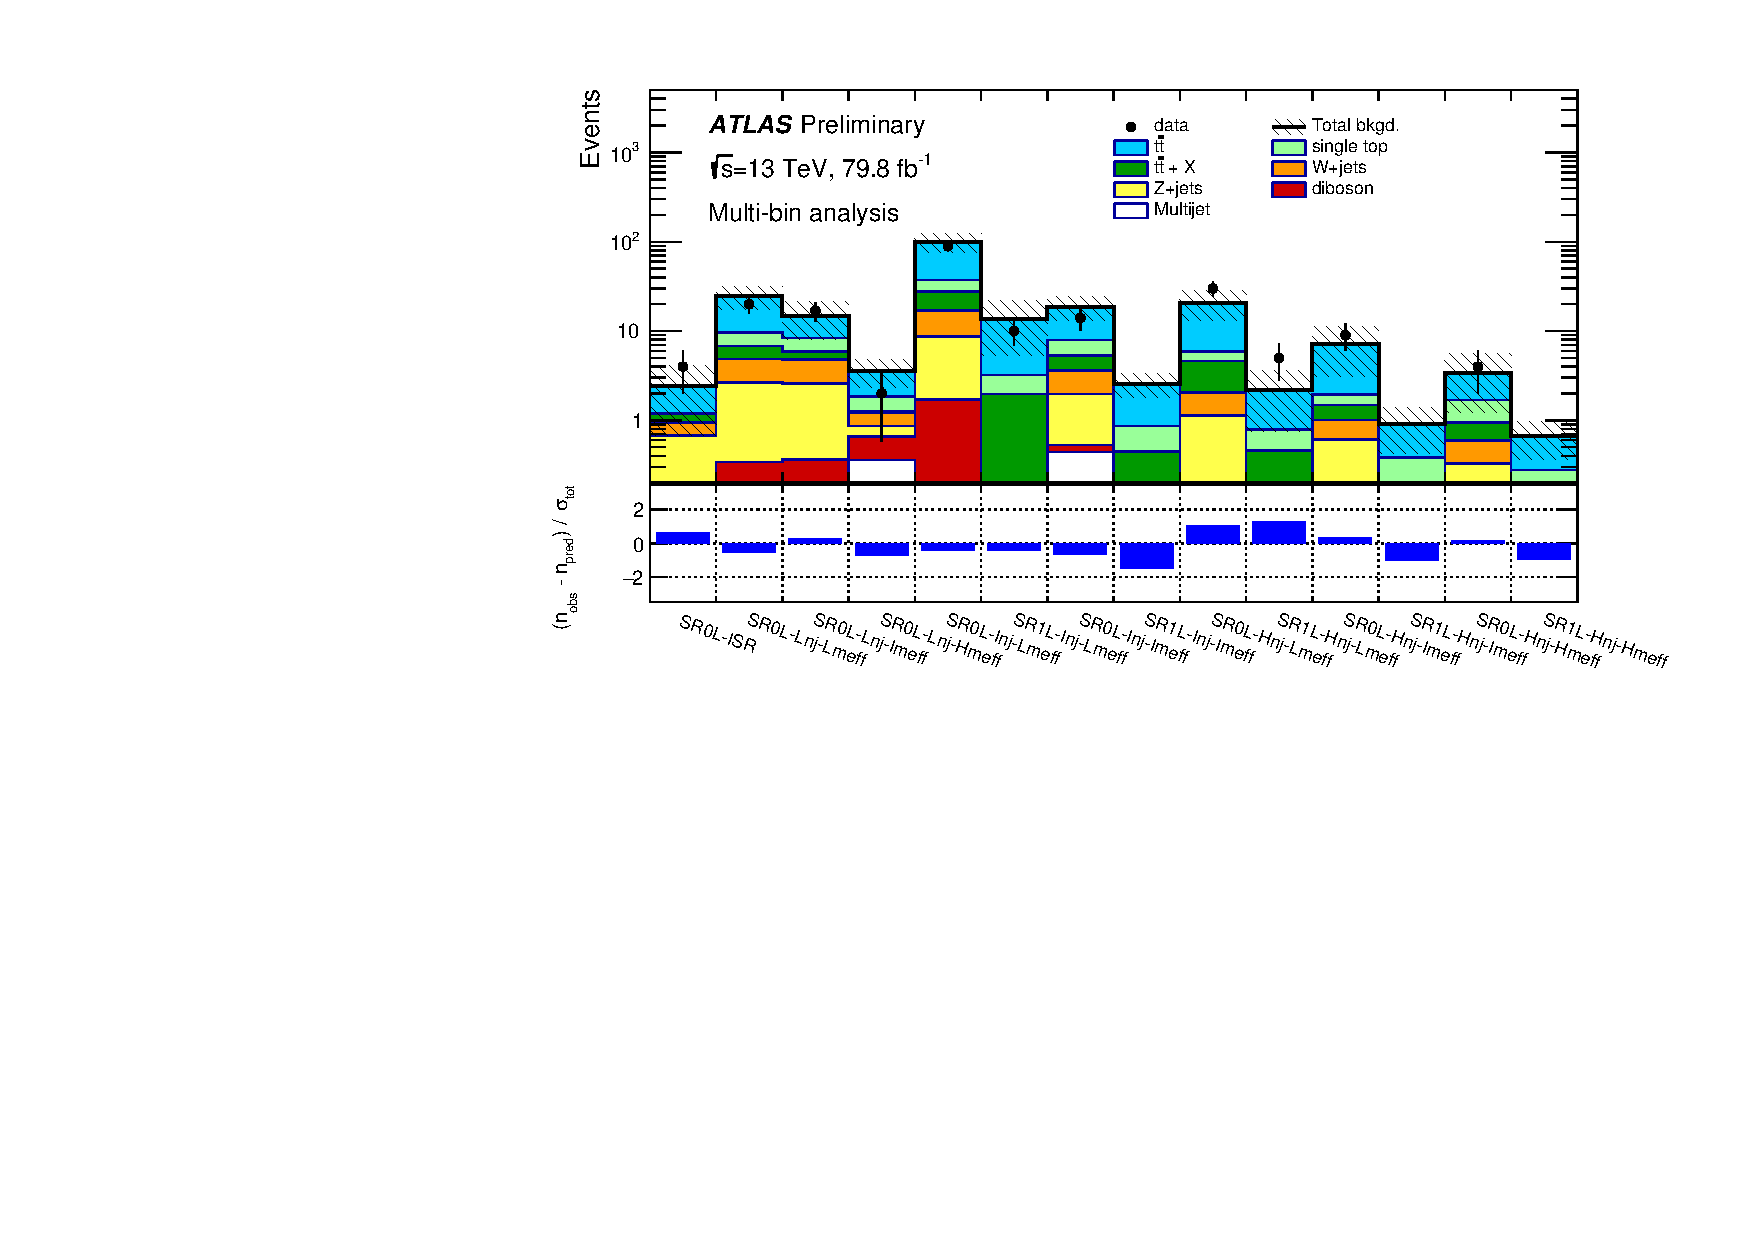
\includegraphics[width=0.9\textwidth]{figures/strong_prod/R21/multibin/histpull_grouping_SR.pdf}\label{fig:pullSR_R21}}\\
	\caption{Results of the background-only fit extrapolated to the \glspl{vr} for \subref{fig:pullVR_R21}
	 and to the \glspl{sr} \subref{fig:pullSR_R21} of the multi-bin analyses. 
	 The data in the  SRs are not included in the fit.  
	 The upper panel shows the observed number of events and the predicted background 
	yield. All the experimental and modelling uncertainties as defined in Ref. \cite{ATLAS-CONF-2018-041} are included in the uncertainty band. 
	The background 
	category $\ttbar+X$ includes $\ttbar W/Z$, $\ttbar H$ and $\ttbar \ttbar$ events. The lower panel shows the 
	pull in each region.} %\temp{The style of the figure will be improved.}} 
	\label{fig:pullR21}
\end{figure}

\subsection{Interpretation}

In this section, we show the model-dependent limits obtained with the update of the multi-bin analysis to include 79.8 \ifb of data. 
